\documentclass[12pt]{article}
\usepackage{verbatim}
\usepackage[dvips]{epsfig}
\usepackage{color}
\usepackage{url}
\usepackage[colorlinks=true]{hyperref}

\begin{document}

\section*{GENESIS: Documentation}

{\bf Related Documentation:}
% start: userdocs-tag-replace-items related-related-add-functionality
% end: userdocs-tag-replace-items related-related-add-functionality

\section*{Create Heccer Test}

Here we describe how to create a test for the {\bf Heccer} package. Since {\bf Heccer} and it's associated simulation objects are all compiled into a library, programs are written in C and compiled against this library to test each use case. In this example, we create suitable tests for the {\it PulseGen\{\}} \href{../simulation-objects/simulation-objects.tex}{\bf Simulation\,Object} ({\it simobj\_PulseGen\{\}}) described in \href{../genesis-add-object-solver/genesis-add-object-solver.tex}{\bf Create\,Solver\,Object}.

\subsection*{Source Files}

The source files for the {\bf Heccer} tests are found in the {\it tests/code} directory within the {\bf Heccer} \href{../reserved-words/reserved-words.tex}{\bf Component}.

\subsection*{Adding an object to the test framework}

Since we are testing a new simulation object, the test framework must be made `aware' of it. A line must be added to each of the files:
\begin{verbatim}
   tests/code/main.c
   tests/code/main.h
\end{verbatim}

In {\it tests/code/main.c} we add:

\begin{verbatim}
   struct simobj_PulseGen *ppg = NULL;
\end{verbatim}

Then in {\it tests/code/main.h} we add:

\begin{verbatim}
   extern struct simobj_PulseGen *ppg;
\end{verbatim}

The main driver for the test framework will now be aware of the {\it PulseGen\{\}} simulation object. Next a source file is created that demonstrates a specific use case.

\subsection*{Use Case}

Ideally, output should be tested against a use case that can be verified to work correctly. Since the {\it PulseGen\{\}} object is a port of the same object used by GENESIS 2, we can obtain output from a GENESIS 2 script to compare with the output of our simulation object.

To test {\it PulseGen\{\}} we want a very basic script that will test minimal functionality in each of its trigger modes. Here is an example that creates three {\it PulseGen\{\}} objects, one for each trigger mode, and sends outputs to a file:
\begin{verbatim}
   create pulsegen /pulse0
   setfield ^ level1 50.0 width1 3.0 delay1 5.0 level2 -20.0 width2 5.0 delay2 8.0 baselevel 10.0 trig_mode 0

   create pulsegen /pulse1
   setfield ^ level1 50.0 width1 3.0 delay1 5.0 level2 -20.0 width2 5.0 delay2 8.0 baselevel 10.0 trig_mode 1

   create pulsegen /pulse2
   setfield ^ level1 50.0 width1 3.0 delay1 5.0 level2 -20.0 width2 5.0 delay2 8.0 baselevel 10.0 trig_mode 2

   create asc_file /pulse0_out 
   setfield /pulse0_out filename "pulse-freerun.txt" flush 1 leave_open 1 append 1 float_format \%0.9g
   addmsg /pulse0 /pulse0_out SAVE output
   call /pulse0_out OUT_OPEN

   create asc_file /pulse1_out 
   setfield /pulse1_out filename "pulse-exttrig.txt" flush 1 leave_open 1 append 1 float_format \%0.9g
   addmsg /pulse1 /pulse1_out SAVE output
   call /pulse1_out OUT_OPEN

   create asc_file /pulse2_out 
   setfield /pulse2_out filename "pulse-extgate.txt" flush 1 leave_open 1 append 1 float_format \%0.9g
   addmsg /pulse2 /pulse2_out SAVE output
   call /pulse2_out OUT_OPEN

   reset
   setclock 0 0.5
   step 200
\end{verbatim}

From data output files we can see what the behavior of the object is supposed to be like.

\begin{figure}[ht]
  \centering
    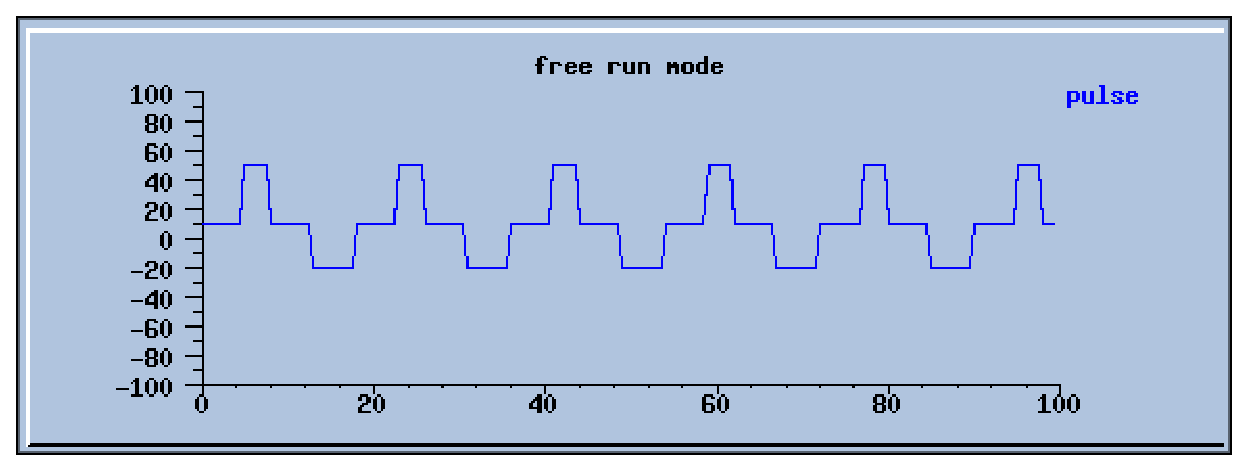
\includegraphics[scale=0.6]{figures/pulse0.eps}
  \caption{Free run mode.}
 % \label{fig:cbi-arch}
\end{figure}

\begin{figure}[ht]
  \centering
    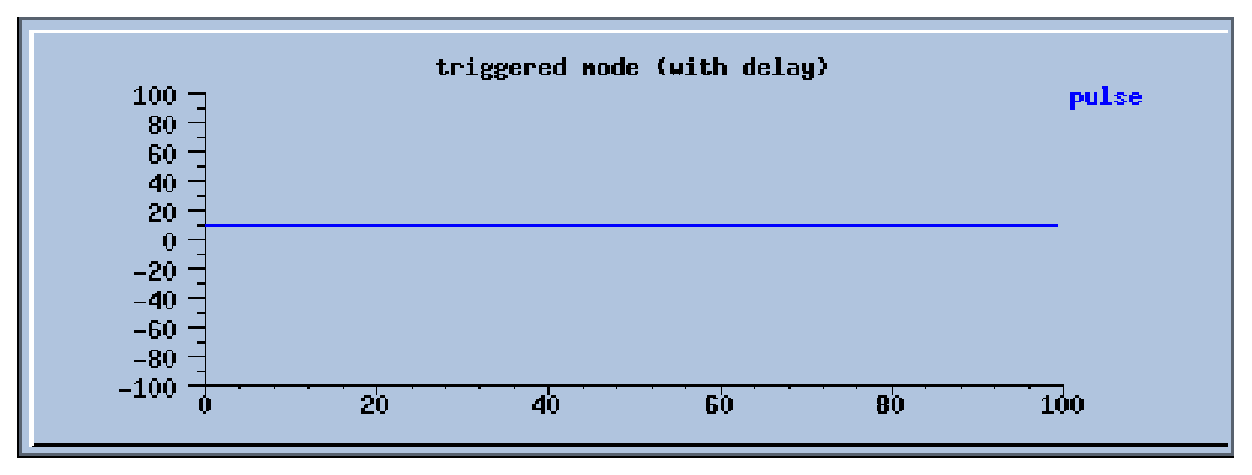
\includegraphics[scale=0.6]{figures/pulse1.eps}
  \caption{External Trigger constant, never triggered.}
 % \label{fig:cbi-arch}
\end{figure}

\begin{figure}[ht]
  \centering
    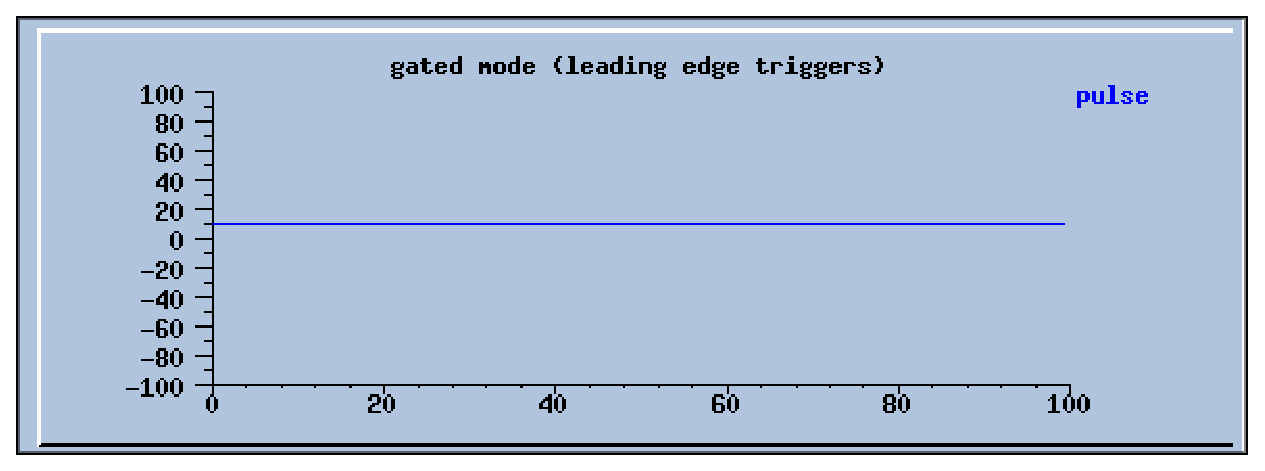
\includegraphics[scale=0.6]{figures/pulse2.eps}
  \caption{External Gate constant, never triggered.}
 % \label{fig:cbi-arch}
\end{figure}

When we run our corresponding {\it PulseGen\{\}} tests we match the value from the solved variable ({\it pdVms0}) for each time step and see that it matches the output we obtain from the GENESIS 2 script. We therefore know this use case works and can set the expected output for the test specification to the output of our program. This serves as a good base case for testing. If these tests should happen to fail then we know some necessary functionality has been compromised during the development of new use cases.

\subsection*{Creating a test program}

A test program for {\bf Heccer} consists of a set of defines, structures, and a main function. Simply changing sections of an existing program is enough to get the test running. The code in each test has inline comments to help understand the functionality, but we'll go through it to be thorough.

At the top of the file you will see defines for setting some simulation and output parameters. Here are some available options:

\begin{itemize}
   \item[]{\bf HECCER\_DUMP\_VM\_COMPARTMENT\_MATRIX} \\
      Output compartment matrix data for solved variables.

   \item[]{\bf HECCER\_DUMP\_VM\_COMPARTMENT\_MATRIX\_DIAGONALS} \\
      Output compartment matrix diagonals for solved variables.

   \item[]{\bf HECCER\_DUMP\_VM\_COMPARTMENT\_OPERATIONS} \\
      Output compartment operations for solved vaiables.

   \item[]{\bf HECCER\_DUMP\_VM\_MECHANISM\_DATA} \\
      Output the mechanism data for solved variables.

   \item[]{\bf HECCER\_DUMP\_VM\_MECHANISM\_OPERATIONS} \\
      Output mechanism operation data for solved variables.

   \item[]{\bf HECCER\_DUMP\_VM\_SUMMARY} \\
      Output run data for solved variables.

   \item[]{\bf HECCER\_TEST\_REPORTING\_GRANULARITY} \\
      This sets the output granularity. In this case the granularity is 1, so our test program will output at every simulation time step. If you want the program to output at every 10th step you can set it to 10, and so on.

   \item[]{\bf HECCER\_TEST\_STEPS} \\
      This is the number of time steps for your simulation.

   \item[]{\bf HECCER\_TEST\_TESTED\_THINGS} \\
      Allows you to output {\bf Heccer} internal data for debugging.

   \item[]{\bf HECCER\_TEST\_TIME\_STEP} \\
      The time step size to use when running the simulation.
\end{itemize}

So here are the settings for our test:
\begin{verbatim}
   #define HECCER_TEST_REPORTING_GRANULARITY 1
   #define HECCER_TEST_STEPS 200
   #define HECCER_TEST_TESTED_THINGS ( HECCER_DUMP_VM_COMPARTMENT_MATRIX | HECCER_DUMP_VM_MECHANISM_OPERATIONS )
   #define HECCER_TEST_TIME_STEP (0.5)
\end{verbatim}
The test will run for 200 steps with a time step of 0.5 seconds. It will produce output, complete with {\bf Heccer} internal data, for every single step of the simulation.

Next, some declarations for data structures that the test will operate on are shown.

We now declare a {\it Compartment\{\}} struct. As the $V_m$ variable (membrane potential) is addressed to produce output, the {\it PulseGen\{\}} object needs the {\it Compartment\{\}} declaration even although it does not perform any compartment specific operations:
\begin{verbatim}
   struct Compartment compSoma =
   {
      //m administrative overhead

      {
         //m type of structure

         MATH_TYPE_Compartment,
      },

      //m index of parent compartment, -1 for none
      -1,

      //m descriptive values, alphabetical order
      /* double dCm; */
      4.57537e-11, // unscaled 0.0164,

      /* double dEm; */
      -0.08,

      /* double dInitVm; */
      -0.068,

      /* double dInject; */
      0,

      /* double dRa; */
      360502, // unscaled 2.5,

      /* double dRm; */
      3.58441e+08, // unscaled 1
};
\end{verbatim}

These declarations set this {\it Compartment\{\}} to be a Math type with no parent, $C_m$ to 4.57537e$^{-11}$, $E_m$ to -0.08, initial membrane potential to -0.068, inject to 0, $R_a$ to 360502, and $R_m$ to 3.58441e$^{+08}$, respectively.

Then an intermediary is declared. Here, the default is used as the test will only use one compartment with one intermediary:
\begin{verbatim}
   int piC2m[] =
   {
      0,
      -1,
   };

   struct Intermediary inter =
   {
      //m compartment array

      1,

      &compSoma,

      //m all other mathematical components

      NULL,

      //m compartment 2 first mechanism number

      piC2m,
};
\end{verbatim}

Next, the main function that actually uses the functions in the simulation object is given. Here a {\it PulseGen\{\}} object is created and its parameters set. This is followed by two {\it \#define}\,s, one to connect the {\it PulseGen\{\}} object to a compartment variable, the other to perform a simulation update time step.

Allocating a new {\it PulseGen\{\}}  is done via:
\begin{verbatim}
   ppg = PulseGenNew("pulsegen freerun");
\end{verbatim}
The parameters of {\it PulseGen\{\}} are then set with the {\it PulseGenSetFields()} function:
\begin{verbatim}
   double dLevel1 = 50.0;
   double dWidth1 = 3.0;
   double dDelay1 = 5.0;
    
   double dLevel2 = -20.0;
   double dWidth2 = 5.0;
   double dDelay2 = 8.0;

   double dBaseLevel = 10.0;

   int iTriggerMode = FREE_RUN;

   PulseGenSetFields(ppg, dLevel1, dWidth2, dDelay1, dLevel2, dWidth2, dDelay2, dBaseLevel, iTriggerMode);   
\end{verbatim}

Next, for the define {\tt HECCER\_TEST\_INITIATE} we fetch a compartment variable from {\bf Heccer} and attach it to the  {\it PulseGen\{\}} output:
\begin{verbatim}
   #define HECCER_TEST_INITIATE \
      double *pdVm = HeccerAddressCompartmentVariable(pheccer, 0, "Vm");  \
      PulseGenAddVariable(ppg, pdVm)
\end{verbatim}
Finally, for {\tt HECCER\_TEST\_SCHEDULE} we add the {\it PulseGen()} step function so that it is performed on every step of the simulation:
\begin{verbatim}
   #define HECCER_TEST_SCHEDULE PulseGenSingleStep(ppg, (dSimulationTime))
\end{verbatim}

\subsection*{Adding source files to the build}

The {\it tests/code} directory has a {\it Makefile.am} which {\it automake} uses to generate a {\it Makefile} for building each test program. We only need to add some information to a couple of places and {\it automake} will handle the rest.

In the target {\it check\_PROGRAMS} we need to add the resulting executable for our test program. For the case {\it pulsegen-freerun.c} we add:
\begin{verbatim}
   pulsegen-freerun \
\end{verbatim}
Next we add rules near the bottom of the file to build and link our program. It is preferable to keep this in alphabetical order with the rest of the test programs build rules:
\begin{verbatim}
   pulsegen_freerun_DEPENDENCIES = ../../libheccer.a main.c
   pulsegen_freerun_LDADD = -L../.. -lheccer -lm
\end{verbatim}
This must be done for each test we want to add.

{\bf Note:} As defined in the first target, the resulting executable is called {\it pulsegen-freerun}. However, to declare the accompanying build rule you must use an underscore, e.g. {\it pulsegen\_freerun}.

\subsection*{Adding a Test Specification}

The final step is to declare a test specification which tests the new test program against output that is known to be correct.

Create the file {\it tests/specifications/pulsegen.t} and input the following to test the {\it pulsegen-freerun} test program. This assumes that the expected output is in the {\it tests/specifications/strings} directory with the filename {\it pulsegen-freerun.txt}.
\begin{verbatim}
#!/usr/bin/perl -w
#

use strict;

my $test
   = {
      command_definitions => [
         {
            arguments => [
            ],
            command => 'tests/code/pulsegen-freerun',
            command_tests => [
               {
                  description => "Can a single pulsegen object output amplitude in free run mode ?",
                  read => (join '', `cat $::config->{core_directory}/tests/specifications/strings/pulsegen-freerun.txt`),
               },
            ],
            description => "pulsegen functionality, can we output a current in free run mode?",
         },
      ],
      description => "pulsegen simulation object",
      name => 'pulsegen.t',
   };
   return $test;
\end{verbatim}
For more information on declaring test specifications see \href{../neurospaces-tester/neurospaces-tester.tex}{\bf Neurospaces Tester}.
 
\end{document}
